\documentclass[tikz, border=10pt]{standalone}
\tikzset{
    vertex/.style = {
        circle,
        fill            = black,
        outer sep = 4pt,
        inner sep = 4pt,
    }
}
\begin{document}
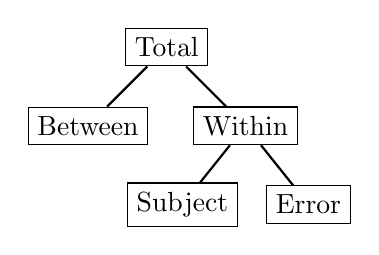
\begin{tikzpicture}
  \node[draw] (Total) at (0,0) {Total};

  \node[draw] (Between) at (-1,-1) {Between};
  \node[draw] (Within) at (1,-1) {Within};

 \node[draw] (Subject) at (0.2,-2) {Subject};
 \node[draw] (Error) at (1.8,-2) {Error};
   
 \draw[->,thick,-] (Total) to (Between);
 \draw[->,thick,-] (Total) to (Within);

 \draw[->,thick,-] (Within) to (Subject);
 \draw[->,thick,-] (Within) to (Error);
  
\end{tikzpicture}
\end{document}